
% !TeX program = xelatex
% !TEX root = main.tex
% !TeX encoding = UTF-8
\documentclass[10.5pt,compsoc]{CjC}
%\usepackage{CJKutf8}
%\usepackage{CJK}
\usepackage{graphicx}
\usepackage{footmisc}
\usepackage{subfigure}
\usepackage{url}
\usepackage{multirow}
\usepackage[noadjust]{cite}
\usepackage{amsmath,amsthm}
\usepackage{amssymb,amsfonts}
\usepackage{booktabs}
\usepackage{color}
\usepackage{ccaption}
\usepackage{booktabs}
\usepackage{float}
\usepackage{fancyhdr}
\usepackage{caption}
\usepackage{xcolor,stfloats}
\usepackage{comment}
\setcounter{page}{1}
\graphicspath{{figures/}}
\usepackage{cuted}%flushend,
\usepackage{captionhack}
\usepackage{epstopdf}
%\usepackage{ccmap}
%\CJKtilde
%\usepackage{CJKpunct} 
%\usepackage[lite,subscriptcorrection,slantedGreek,nofontinfo]{mtpro2}

%===============================%

%\firstfootname{ \quad \quad }
\headevenname{\mbox{\quad} \hfill  \mbox{\zihao{-5}{\songti  计\quad \quad 算\quad \quad 机\quad \quad 学\quad \quad 报 } \hspace {50mm} \mbox{\songti  2019 年 }}}%
\headoddname{\songti  ? 期 \hfill
作者姓名等:论文题目 }%

%footnote use of *
\renewcommand{\thefootnote}{\fnsymbol{footnote}}
\setcounter{footnote}{0}
\renewcommand\footnotelayout{\zihao{5-}}

\newtheoremstyle{mystyle}{0pt}{0pt}{\normalfont}{1em}{\bf}{}{1em}{}
\theoremstyle{mystyle}
\renewcommand\figurename{figure~}
\renewcommand{\thesubfigure}{(\alph{subfigure})}
\newcommand{\upcite}[1]{\textsuperscript{\cite{#1}}}
\renewcommand{\labelenumi}{(\arabic{enumi})}
\newcommand{\tabincell}[2]{\begin{tabular}{@{}#1@{}}#2\end{tabular}}
\newcommand{\abc}{\color{white}\vrule width 2pt}
\makeatletter
\renewcommand{\@biblabel}[1]{[#1]\hfill}
\makeatother
\setlength\parindent{2em}
%\renewcommand{\hth}{\heiti }
%\renewcommand{\htss}{\begin{CJK*}{UTF8}{song}}


\begin{document}
\hyphenpenalty=50000
\makeatletter
\newcommand\mysmall{\@setfontsize\mysmall{7}{9.5}}
\newenvironment{tablehere}
  {\def\@captype{table}}

\let\temp\footnote
\renewcommand \footnote[1]{\temp{\zihao{-5}#1}}


\thispagestyle{plain}%
\thispagestyle{empty}%
\pagestyle{CjCheadings}

\begin{table*}[!t]
\vspace {-13mm}
\begin{tabular}{p{168mm}}
\zihao{5-}
\songti 
神经网络理论与应用课程大作业\quad \quad 学号:921000912028\quad \quad 姓名:翁创\quad \quad 2022年5月 \\
\hline\\[-4.5mm]
\hline\end{tabular}

\centering
\vspace{11mm}
\heiti  
{\zihao{2} 题目(中英文题目一致)字体为2号黑体(全文除特别声明外, 外文统一用Times New Roman) }

\vskip 5mm

{\zihao{3} \fangsong 
作者名$^{1)}$\quad  作者名$^{2),3)}$ \quad 作者名$^{3) }$($^*$字体为3号仿宋*作者)
 }

\vspace{5mm}
\zihao{6}{\songti 
$^{1)}$(单位全名 部门(系)全名, 市(或直辖市) 国家名 邮政编码)
*字体为6号宋体*单位
 }

\zihao{6}{\songti  
$^{2)}$(单位全名 部门(系)全名, 市(或直辖市) 国家名
邮政编码)*中英文单位名称、作者姓名须一致*}

\zihao{6}{\songti  
$^{3)}$(单位全名 部门(系)全名, 市(或直辖市) 国家名 邮政编码)
 }

\zihao{6}{\heiti 
论文定稿后,作者署名、单位无特殊情况不能变更。若变更,须提交签章申请,国家名为中国可以不写,省会城市不写省的名称,其他国家必须写国家名。
 }

\vskip 5mm
{\centering
\begin{tabular}{p{160mm}}
\zihao{5-}{
\setlength{\baselineskip}{16pt}\selectfont{
\noindent\heiti 摘\quad 要\quad   \songti  
*中文摘要内容置于此处(英文摘要中要有这些内容),字体为小5号宋体。摘要贡献部分,要有数据支持,不要出现``...大大提高''、``...显著改善''等描述,正确的描述是``比{\ldots}提高X{\%}''、
``在{\ldots}上改善X{\%}''。*摘要

 \par}}\\[2mm]

\zihao{5-}{\noindent
\heiti 关键词  \quad \songti  {*关键词(中文关键字与英文关键字对应且一致,应有5-7个关键词);关键词;关键词;关键词*  }
 
}\\[2mm]
\zihao{5-}{\heiti 中图法分类号 	\songti  
TP \rm{\quad \quad \quad     }
\heiti DOI号: \songti  
*投稿时不提供DOI号 }
\end{tabular}}

\vskip 7mm

\begin{center}
\zihao{3}{ {\heiti Title *(中英文题目一致)字体为4号Times New Roman,加粗* Title }}\\
\vspace {5mm}
\zihao{5}{ {\heiti NAME Name-Name$^{1)}$ NAME Name$^{2)}$ NAME Name-Name$^{3)}$ *字体为5号Times
new Roman*Name 
}}\\
\vspace {2mm}
\zihao{6}{\heiti {$^{1)}$(Department of ****, University, City ZipCode, China) *字体为6号Times
new Roman* Depart.Correspond} }

\zihao{6}{\heiti {$^{2)}$(Department of ****, University, City ZipCode)*中国不写国家名*} }

\zihao{6}{\heiti {$^{3)}$(Department of ****, University, City ZipCode, country)*外国写国家名*} }



\end{center}

\begin{tabular}{p{160mm}}
\zihao{5}{
\setlength{\baselineskip}{18pt}\selectfont{
{\bf Abstract}\quad \begin{heiti} (\textbf{500英文单词,内容包含中文摘要的内容}).
字体为Times new Roman,字号5号* Abstract \end{heiti}
\par}}\\

\setlength{\baselineskip}{18pt}\selectfont{
\zihao{5}{\noindent Do not modify the amount of space before and after the artworks. One- or two-column format artworks are preferred. and Tables, create a new break line and paste the resized artworks where desired. Do not modify the amount of space before and after the artworks. One- or two-column format artworks are preferred. All Schemes, Equations, Figures, and Tables should be mentioned in the text consecutively and numbered with Arabic numerals, and appear below where they are mentioned for the first time in the main text. To insert Schemes, Equations, Figures, and Tables, create a new break line and paste the resized artworks where desired. Do not modify the amount of space before and after the artworks. One- or two-column format artworks are preferred.Do not modify the amount of space before and after the artworks. One- or two-column format artworks are preferred. and Tables, create a new break line and paste the resized artworks where desired. Do not modify the amount of space before and after the artworks. One- or two-column format artworks are preferred. All Schemes, Equations, Figures, and Tables should be mentioned in the text consecutively and numbered with Arabic numerals, and appear below where they are mentioned for the first time in the main text.

\vspace {5mm}
{\bf Keywords}\quad \heiti 中文关键字与英文关键字对应且一致,\textbf{不要用英文缩写});
key word; key word; key word* *字体为5号Times new Roman * Key words }\par}
\end{tabular}

\setlength{\tabcolsep}{2pt}
\end{table*}
\clearpage\clearpage
\begin{strip}
\vspace {-13mm}
\end{strip}
    \linespread{1.15}
\heiti 
\zihao{5}
\vskip 1mm
\section{长短时记忆网络原理}
{\heiti \subsection{长短时记忆网络的前向计算} }

\songti
前面描述的开关是怎样在算法中实现的呢? 这就用到了门 ( gate) 的概念。 门实际上就是一层全连接层,它的输入是一个向量,输出是一个 0到1之间的实数向量。假设W是门的权重向量,  是偏置项,那么门可以表示为:
$$
g(\mathbf{x})=\sigma(W \mathbf{x}+\mathbf{b})
$$

门的使用,就是用门的输出向量按元素乘以我们需要控制的那个向量。因为门的输出是0到1之间的实数向量,那么,当门输出为 0 时,任何 向量与之相乘都会得到 0 向量,这就相当于咶都不能通过;输出为1时,任何向量与之相乘都不会有任何改变,这就相当于啥都可以通过。因 为 $\sigma$ (也就是sigmoid函数) 的值域是 $(0,1)$ ,所以门的状态都是半开半闭的。

LSTM用两个门来控制单元状态c的内容,一个是遗忘门 ( forget gate),它决定了上一时刻的单元状态 $\mathbf{c}_{t-1}$ 有多少保留到当前时刻 $\mathbf{c}_{t}$; 另 个个是输入门 ( input gate ),它决定了当前时刻网络的输入 $\mathbf{x}_{t}$ 有多少保存到单元状态 $\mathbf{c}_{t}$ 。LSTM用输出门 (output gate ) 来控制单元状 态 $\mathbf{c}_{t}$ 有多少输出到LSTM的当前输出值 $\mathbf{h}_{t}$ 。

我们先来看一下遗忘门:
$$
\mathbf{f}_{t}=\sigma\left(W_{f} \cdot\left[\mathbf{h}_{t-1}, \mathbf{x}_{t}\right]+\mathbf{b}_{f}\right)
$$
上式中, $W_{f}$ 是遗忘门的权重矩阵, $\left[\mathbf{h}_{t-1}, \mathbf{x}_{t}\right]$ 表示把两个向量连接成一个更长的向量, $\mathbf{b}_{f}$ 是遗忘门的偏置项, $\sigma$ 是sigmoid函数。如果输 入的维度是 $d_{x}$ ,隐藏层的维度是 $d_{h}$ ,单元状态的维度是 $d_{c}$ (通常 $d_{c}=d_{h}$ ),则遗忘门的权重矩阵 $W_{f}$ 维度是 $d_{c} \times\left(d_{h}+d_{x}\right)$ 。事实 上,权重矩阵 $W_{f}$ 都是两个矩阵拼接而成的: 个个是 $W_{f h}$ ,它对应着输入项 $\mathbf{h}_{t-1}$ ,其维度为 $d_{c} \times d_{h} ;$ 个是 $W_{f x}$ ,它对应着输入项 $\mathbf{x}_{t}$ , 其维度为 $d_{c} \times d_{x}$ 。 $W_{f}$ 可以写为 :
$$
\begin{aligned}
{\left[W_{f}\right]\left[\begin{array}{c}
\mathbf{h}_{t-1} \\
\mathbf{x}_{t}
\end{array}\right] } &=\left[\begin{array}{ll}
W_{f h} & W_{f x}
\end{array}\right]\left[\begin{array}{c}
\mathbf{h}_{t-1} \\
\mathbf{x}_{t}
\end{array}\right] \\
&=W_{f h} \mathbf{h}_{t-1}+W_{f x} \mathbf{x}_{t}
\end{aligned}
$$

下图显示了遗忘门的计算 :

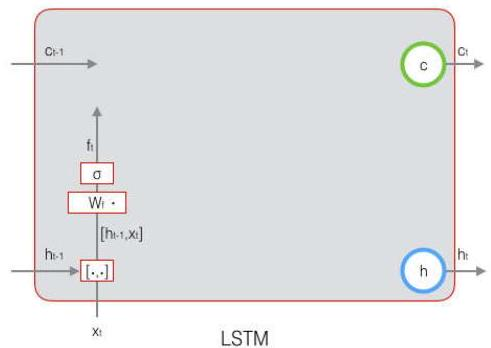
\includegraphics[width=6cm, height=4cm]{images/2022_05_03_e4231fc9c1842f38b0acg-03(1)}

接下来看看输入门:
$$
\mathbf{i}_{t}=\sigma\left(W_{i} \cdot\left[\mathbf{h}_{t-1}, \mathbf{x}_{t}\right]+\mathbf{b}_{i}\right)
$$

上式中, $W_{i}$ 是输入门的权重矩阵, $\mathbf{b}_{i}$ 是输入门的偏置项。下图表示了输入门的计算 :

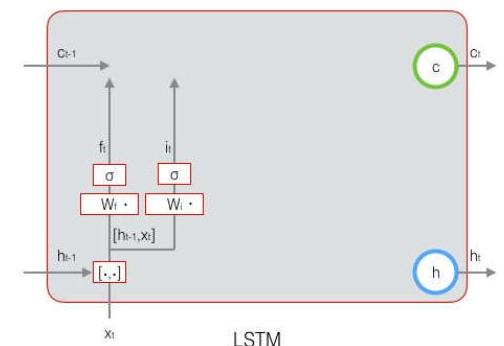
\includegraphics[width=6cm, height=4cm]{images/2022_05_03_e4231fc9c1842f38b0acg-04}

接下来,我们计算用于描述当前输入的单元状态 $\boldsymbol{c}_{t}$ ,它是根据上一次的输出和本次输入来计算的:
$$
\tilde{\mathbf{c}}_{t}=\tanh \left(W_{c} \cdot\left[\mathbf{h}_{t-1}, \mathbf{x}_{t}\right]+\mathbf{b}_{c}\right)
$$

下图是 $\tilde{c}_{t}$ 的计算 :

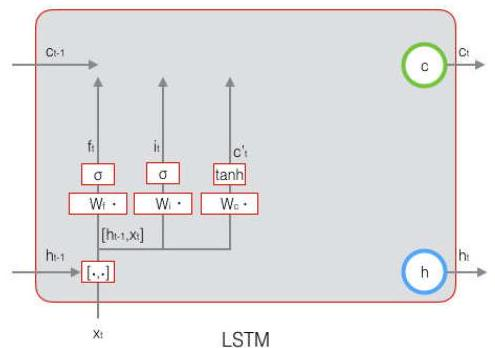
\includegraphics[width=6cm, height=4cm]{images/2022_05_03_e4231fc9c1842f38b0acg-04(1)}

现在,我们计算当前时刻的单元状态 $\mathbf{c}_{t}$ 。它是由上一次的单元状态 $\mathbf{c}_{t-1}$ 按元素乘以遗忘门 $f_{t}$ ,再用当前输入的单元状态 $\tilde{c}_{t}$ 按元素乘以输入 $门 i_{t}$ ,再将两个积加和产生的:
$$
\mathbf{c}_{t}=f_{t} \circ \mathbf{c}_{t-1}+i_{t} \circ \tilde{\mathbf{c}}_{t}
$$

符号○表示按元素乘。下图是 $\mathbf{c}_{t}$ 的计算 :

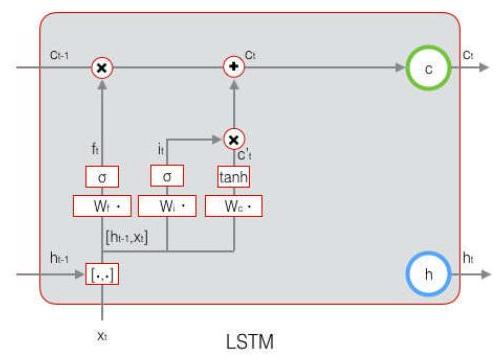
\includegraphics[width=6cm, height=4cm]{images/2022_05_03_e4231fc9c1842f38b0acg-04(2)}

这样,我们就把LSTM关于当前的记忆 $\tilde{c}_{t}$ 和长期的记忆 $\mathbf{c}_{t-1}$ 组合在一起,形成了新的单元状态 $\mathbf{c}_{t}$ 。由于遗忘门的控制,它可以保存很久很久 之前的信息,由于输入门的控制,它又可以避免当前无关紧要的内容进入记忆。下面,我们要看看输出门,它控制了长期记忆对当前输出的 影响 :
$$
\mathbf{o}_{t}=\sigma\left(W_{o} \cdot\left[\mathbf{h}_{t-1}, \mathbf{x}_{t}\right]+\mathbf{b}_{o}\right)
$$

下图表示输出门的计算:

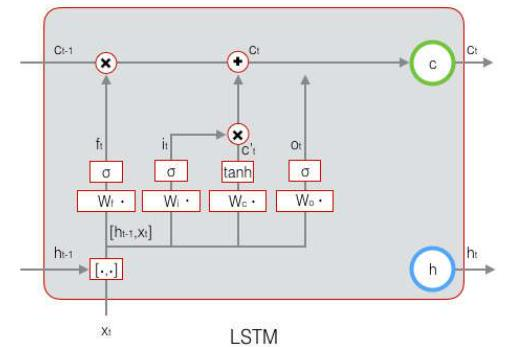
\includegraphics[width=6cm, height=4cm]{images/2022_05_03_e4231fc9c1842f38b0acg-05}

LSTM最终的输出,是由输出门和单元状态共同确定的 :
$$
\mathbf{h}_{t}=\mathbf{o}_{t} \circ \tanh \left(\mathbf{c}_{t}\right)
$$

下图表示LSTM最终输出的计算 :

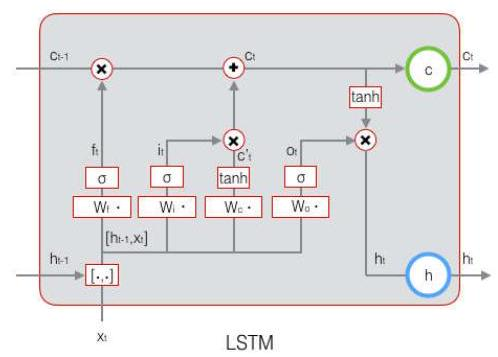
\includegraphics[width=6cm, height=4cm]{images/2022_05_03_e4231fc9c1842f38b0acg-05(1)}

式1到式6就是LSTM前向计算的全部公式。\\

{\heiti \subsection{长短时记忆网络的训练} }
熟悉我们这个系列文章的同学都清楚,训练部分往往比前向计算部分复杂多了。LSTM的前向计算都这么复杂,那么,可想而知,它的训练 算法一定是非常非常复杂的。现在只有做几次深呼吸,再一头扎进公式海洋吧。\\

{\heiti \subsection{LSTM训练算法框架} }
LSTM的训练算法仍然是反向传播算法,对于这个算法,我们已经非常熟悉了。主要有下面三个步骤 :

\begin{enumerate}
  \item 前向计算每个神经元的输出值,对于LSTM来说,即 $\mathbf{f}_{t} 、 \mathbf{i}_{t} 、 \mathbf{c}_{t} 、 \mathbf{o}_{t} 、 \mathbf{h}_{t}$ 五个向量的值。计算方法已经在上一节中描述过了。

  \item 反向计算每个神经元的误差项 $\delta$ 值。与循环神经网络一样,LSTM误差项的反向传播也是包括两个方向 : 一个是沿时间的反向传播,即 从当前时刻开始,计算每个时刻的误差项;一个是将误差项向上一层传播。

\end{enumerate}
{\heiti \subsection{用于公式和符号的说明} }
首先,我们对推导中用到的一些公式、符号做一下必要的说明。

接下来的推导中,我们设定gate的激活函数为sigmoid函数,输出的激活函数为tanh函数。他们的导数分别为:
$$
\begin{aligned}
\sigma(z) &=y=\frac{1}{1+e^{-z}} \\
\sigma^{\prime}(z) &=y(1-y) \\
\tanh (z) &=y=\frac{e^{z}-e^{-z}}{e^{z}+e^{-z}} \\
\tanh ^{\prime}(z) &=1-y^{2}
\end{aligned}
$$

从上面可以看出,sigmoid和tanh函数的导数都是原函数的函数。这样,我们一旦计算原函数的值,就可以用它来计算出导数的值。

LSTM需要学习的参数共有 8 组,分别是 : 遗忘门的权重矩阵 $W_{f}$ 和偏置项 $\mathbf{b}_{f}$ 、输入门的权重矩阵 $W_{i}$ 和偏置项 $\mathbf{b}_{i}$ 、输出门的权重矩阵 $W_{o}$ 和 我们解释一下按元素乘 $@$ 符号。当O作用于两个向量时,运算如下:
$$
\mathbf{a} \circ \mathbf{b}=\left[\begin{array}{c}
a_{1} \\
a_{2} \\
a_{3} \\
\ldots \\
a_{n}
\end{array}\right] \circ\left[\begin{array}{c}
b_{1} \\
b_{2} \\
b_{3} \\
\ldots \\
b_{n}
\end{array}\right]=\left[\begin{array}{c}
a_{1} b_{1} \\
a_{2} b_{2} \\
a_{3} b_{3} \\
\cdots \\
a_{n} b_{n}
\end{array}\right]
$$

当○作用于一个向量和一个矩阵时,运算如下 :
$$
\begin{aligned}
\mathbf{a} \circ X &=\left[\begin{array}{l}
a_{1} \\
a_{2} \\
a_{3} \\
\ldots \\
a_{n}
\end{array}\right] \circ\left[\begin{array}{lllll}
x_{11} & x_{12} & x_{13} & \ldots & x_{1 n} \\
x_{21} & x_{22} & x_{23} & \ldots & x_{2 n} \\
x_{31} & x_{32} & x_{33} & \ldots & x_{3 n} \\
& & \ldots & & \\
x_{n 1} & x_{n 2} & x_{n 3} & \ldots & x_{n n}
\end{array}\right] \\
=& {\left[\begin{array}{llllll}
a_{1} x_{11} & a_{1} x_{12} & a_{1} x_{13} & \ldots & a_{1} x_{1 n} \\
a_{2} x_{21} & a_{2} x_{22} & a_{2} x_{23} & \ldots & a_{2} x_{2 n} \\
a_{3} x_{31} & a_{3} x_{32} & a_{3} x_{33} & \ldots & a_{3} x_{3 n} \\
a_{n} x_{n 1} & a_{n} x_{n 2} & a_{n} x_{n 3} & \ldots & a_{n} x_{n n}
\end{array}\right] }
\end{aligned}
$$

当○作用于两个矩阵时,两个矩阵对应位置的元素相乘。按元素乘可以在某些情况下简化矩阵和向量运算。例如,当一个对角矩阵右乘一个 矩阵时,相当于用对角矩阵的对角线组成的向量按元素乘那个矩阵 :
$$
\operatorname{diag}[\mathbf{a}] X=\mathbf{a} \circ X
$$

当一个行向量右乘一个对角矩阵时,相当于这个行向量按元素乘那个矩阵对角线组成的向量 :
$$
\mathbf{a}^{T} \operatorname{diag}[\mathbf{b}]=\mathbf{a} \circ \mathbf{b}
$$

上面这两点,在我们后续推导中会多次用到。

在t时刻,LSTM的输出值为 $\mathbf{h}_{t}$ 。我们定义时刻的误差项 $\delta_{t}$ 为 :
$$
\delta_{t} \stackrel{\text { def }}{=} \frac{\partial E}{\partial \mathbf{h}_{t}}
$$

注意,和前面几篇文章不同,我们这里假设误差项是损失函数对输出值的导数,而不是对加权输入net $t_{t}^{l}$ 的导数。因为LSTM有四个加权输 入,分别对应 $\mathbf{f}_{t} 、 \mathbf{i}_{t} 、 \mathbf{c}_{t} 、 \mathbf{o}_{t}$ ,我们希望往上一层传递一个误差项而不是四个。但我们仍然需要定义出这四个加权输入,以及他们对应的误 差项。
$$
\begin{aligned}
\mathbf{n e t}_{f, t} &=W_{f}\left[\mathbf{h}_{t-1}, \mathbf{x}_{t}\right]+\mathbf{b}_{f} \\
&=W_{f h} \mathbf{h}_{t-1}+W_{f x} \mathbf{x}_{t}+\mathbf{b}_{f} \\
\mathbf{n e t}_{i, t} &=W_{i}\left[\mathbf{h}_{t-1}, \mathbf{x}_{t}\right]+\mathbf{b}_{i} \\
&=W_{i h} \mathbf{h}_{t-1}+W_{i x} \mathbf{x}_{t}+\mathbf{b}_{i} \\
\mathbf{n e t}_{\tilde{c}, t} &=W_{c}\left[\mathbf{h}_{t-1}, \mathbf{x}_{t}\right]+\mathbf{b}_{c} \\
&=W_{c h} \mathbf{h}_{t-1}+W_{c x} \mathbf{x}_{t}+\mathbf{b}_{c} \\
\mathbf{n e t}_{o, t} &=W_{o}\left[\mathbf{h}_{t-1}, \mathbf{x}_{t}\right]+\mathbf{b}_{o} \\
&=W_{o h} \mathbf{h}_{t-1}+W_{o x} \mathbf{x}_{t}+\mathbf{b}_{o} \\
\delta_{f, t} & \stackrel{\text { def }}{=} \frac{\partial E}{\partial \mathbf{n e t}_{f, t}} \\
\delta_{i, t} & \stackrel{\text { def }}{=} \frac{\partial E}{\partial \mathbf{n e t}}{ }_{i, t} \\
\delta_{\tilde{c}, t} & \stackrel{\text { def }}{=} \frac{\partial E}{\partial \mathbf{n e t}_{\tilde{c}, t}} \\
\delta_{o, t} & \stackrel{\text { def }}{=} \frac{\partial E}{\partial \mathbf{n e t}_{o, t}}
\end{aligned}
$$

{\heiti \subsection{误差项沿时间的反向传递} }
沿时间反向传递误差项,就是要计算出t-1时刻的误差项 $\delta_{t-1 \text { 。 }}$
$$
\begin{aligned}
\delta_{t-1}^{T} &=\frac{\partial E}{\partial \mathbf{h}_{\mathbf{t}-\mathbf{1}}} \\
&=\frac{\partial E}{\partial \mathbf{h}_{\mathbf{t}}} \frac{\partial \mathbf{h}_{\mathbf{t}}}{\partial \mathbf{h}_{\mathbf{t}-\mathbf{1}}} \\
&=\delta_{t}^{T} \frac{\partial \mathbf{h}_{\mathbf{t}}}{\partial \mathbf{h}_{\mathbf{t}-1}}
\end{aligned}
$$

我们知道, $\frac{\partial \mathbf{h}_{t}}{\partial \mathbf{h}_{t-1}}$ 是一个Jacobian矩阵。如果隐藏层 $h$ 的维度是 $N$ 的话,那么它就是一个 $N \times N$ 矩阵。为了求出它,我们列出 $\mathbf{h}_{t}$ 的计算公 式,即前面的式6和式4 :
$$
\begin{aligned}
&\mathbf{h}_{t}=\mathbf{o}_{t} \circ \tanh \left(\mathbf{c}_{t}\right) \\
&\mathbf{c}_{t}=\mathbf{f}_{t} \circ \mathbf{c}_{t-1}+\mathbf{i}_{t} \circ \tilde{\mathbf{c}}_{t}
\end{aligned}
$$

显然, $\mathbf{o}_{t} 、 \mathbf{f}_{t} 、 \mathbf{i}_{t} 、 \tilde{\mathbf{c}}_{t}$ 都是 $\mathbf{h}_{t-1}$ 的函数,那么,利用全导数公式可得 :
$$
\begin{aligned}
\delta_{t}^{T} \frac{\partial \mathbf{h}_{\mathbf{t}}}{\partial \mathbf{h}_{\mathbf{t}-1}} &=\delta_{t}^{T} \frac{\partial \mathbf{h}_{\mathbf{t}}}{\partial \mathbf{o}_{t}} \frac{\partial \mathbf{o}_{t}}{\partial \mathbf{n e t}_{o, t}} \frac{\partial \mathbf{n e t}_{o, t}}{\partial \mathbf{h}_{\mathbf{t}-\mathbf{1}}}\\
&+\delta_{t}^{T} \frac{\partial \mathbf{h}_{\mathbf{t}}}{\partial \mathbf{c}_{t}} \frac{\partial \mathbf{c}_{t}}{\partial \mathbf{f}_{\mathbf{t}}} \frac{\partial \mathbf{f}_{t}}{\partial \mathbf{n e t}_{f, t}} \frac{\partial \mathbf{n e t}_{f, t}}{\partial \mathbf{h}_{\mathbf{t}-1}}\\
&+\delta_{t}^{T} \frac{\partial \mathbf{h}_{\mathbf{t}}}{\partial \mathbf{c}_{t}} \frac{\partial \mathbf{c}_{t}}{\partial \mathbf{i}_{\mathbf{t}}} \frac{\partial \mathbf{i}_{t}}{\partial \mathbf{n e t}_{i, t}} \frac{\partial \mathbf{n e t}_{i, t}}{\partial \mathbf{h}_{\mathbf{t}-\mathbf{1}}}\\
&+\delta_{t}^{T} \frac{\partial \mathbf{h}_{\mathbf{t}}}{\partial \mathbf{c}_{t}} \frac{\partial \mathbf{c}_{t}}{\partial \tilde{\mathbf{c}}_{t}} \frac{\partial \tilde{\mathbf{c}}_{t}}{\partial \mathbf{n e t}_{\tilde{c}, t}} \\
&=\delta_{o, t}^{T} \frac{\partial \mathbf{n e t}_{o, t}}{\partial \mathbf{h}_{\mathbf{t}-1}}+\delta_{f, t}^{T} \frac{\partial \mathbf{n e t}_{f, t}}{\partial \mathbf{h}_{\mathbf{t}-\mathbf{1}}}\\
&+\delta_{i, t}^{T} \frac{\partial \mathbf{n e t}_{i, t}}{\partial \mathbf{h}_{\mathbf{t}-1}}+\delta_{\tilde{c}, t}^{T} \frac{\partial \mathbf{n e t}_{\tilde{c}, t}}{\partial \mathbf{h}_{\mathbf{t}-\mathbf{1}}}
\end{aligned}
$$

下面,我们要把式7中的每个偏导数都求出来。根据式6,我们可以求出 :
$$
\begin{aligned}
\frac{\partial \mathbf{h}_{\mathbf{t}}}{\partial \mathbf{o}_{t}} &=\operatorname{diag}\left[\tanh \left(\mathbf{c}_{t}\right)\right] \\
\frac{\partial \mathbf{h}_{\mathbf{t}}}{\partial \mathbf{c}_{t}} &=\operatorname{diag}\left[\mathbf{o}_{t} \circ\left(1-\tanh \left(\mathbf{c}_{t}\right)^{2}\right)\right]
\end{aligned}
$$

根据式4,我们可以求出 :
$$
\begin{aligned}
\frac{\partial \mathbf{c}_{t}}{\partial \mathbf{f}_{\mathbf{t}}} &=\operatorname{diag}\left[\mathbf{c}_{t-1}\right] \\
\frac{\partial \mathbf{c}_{t}}{\partial \mathbf{i}_{\mathbf{t}}} &=\operatorname{diag}\left[\tilde{\mathbf{c}}_{t}\right] \\
\frac{\partial \mathbf{c}_{t}}{\partial \tilde{\mathbf{c}}_{\mathbf{t}}} &=\operatorname{diag}\left[\mathbf{i}_{t}\right]
\end{aligned}
$$

因为:
$$
\begin{aligned}
\mathbf{o}_{t} &=\sigma\left(\mathbf{n e t}_{o, t}\right) \\
\mathbf{n e t}_{o, t} &=W_{o h} \mathbf{h}_{t-1}+W_{o x} \mathbf{x}_{t}+\mathbf{b}_{o} \\
\mathbf{f}_{t} &=\sigma\left(\mathbf{n e t}_{f, t}\right) \\
\mathbf{n e t}_{f, t} &=W_{f h} \mathbf{h}_{t-1}+W_{f x} \mathbf{x}_{t}+\mathbf{b}_{f} \\
\mathbf{i}_{t} &=\sigma\left(\mathbf{n e t}_{i, t}\right) \\
\mathbf{n e t}_{i, t} &=W_{i h} \mathbf{h}_{t-1}+W_{i x} \mathbf{x}_{t}+\mathbf{b}_{i} \\
\tilde{\mathbf{c}}_{t} &=\tanh \left(\mathbf{n e t}_{\tilde{c}, t}\right) \\
\mathbf{n e t}_{\tilde{c}, t} &=W_{c h} \mathbf{h}_{t-1}+W_{c x} \mathbf{x}_{t}+\mathbf{b}_{c}
\end{aligned}
$$

我们很容易得出 :
$$
\begin{aligned}
\frac{\partial \mathbf{o}_{t}}{\partial \mathbf{n e t}_{o, t}} &=\operatorname{diag}\left[\mathbf{f}_{t} \circ\left(1-\mathbf{o}_{t}\right)\right]\\
\frac{\partial \mathbf{n e t}_{o, t}}{\partial \mathbf{h}_{\mathbf{t}-\mathbf{1}}} &=W_{o h} \\
\frac{\partial \mathbf{f}_{t}}{\partial \mathbf{n e t}_{f, t}} &=\operatorname{diag}\left[\mathbf{f}_{t} \circ\left(1-\mathbf{f}_{t}\right)\right] \\
\frac{\partial \mathbf{n e t}_{f, t}}{\partial \mathbf{h}_{t-1}} &=W_{f h} \\
\frac{\partial \mathbf{i}_{t}}{\partial \mathbf{n e t}_{i, t}} &=\operatorname{diag}\left[\mathbf{i}_{t} \circ\left(1-\mathbf{i}_{t}\right)\right] \\
\frac{\partial \mathbf{n e t}_{i, t}}{\partial \mathbf{h}_{t-1}} &=W_{i h} \\
\frac{\partial \tilde{\mathbf{c}}_{t}}{\partial \mathbf{n e t}_{\tilde{,}, t}} &=\operatorname{diag}\left[1-\tilde{\mathbf{c}}_{t}^{2}\right] \\
\frac{\partial \mathbf{n e t}_{\tilde{,}, t}}{\partial \mathbf{h}_{t-1}} &=W_{c h}
\end{aligned}
$$

将上述偏导数带入到式7,我们得到 :
$$
\begin{aligned}
\delta_{t-1} &=\delta_{o, t}^{T} \frac{\partial \mathbf{n e t}_{o, t}}{\partial \mathbf{h}_{\mathbf{t}-1}}+\delta_{f, t}^{T} \frac{\partial \mathbf{n e t}_{f, t}}{\partial \mathbf{h}_{\mathbf{t}-1}}+\delta_{i, t}^{T} \frac{\partial \mathbf{n e t}_{i, t}}{\partial \mathbf{h}_{\mathbf{t}-1}}+\delta_{\tilde{c}, t}^{T} \frac{\partial \mathbf{n e t}_{\tilde{c}, t}}{\partial \mathbf{h}_{\mathbf{t}-\mathbf{1}}} \\
&\left.=\delta_{o, t}^{T} W_{o h}+\delta_{f, t}^{T} W_{f h}+\delta_{i, t}^{T} W_{i h}+\delta_{\tilde{c}, t}^{T} W_{c h} \text { (式 } 8\right)
\end{aligned}
$$

根据 $\delta_{o, t} 、 \delta_{f, t} 、 \delta_{i, t} 、 \delta_{\tilde{c}, t}$ 的定义,可知:
$$
\begin{aligned}
\delta_{o, t}^{T} &=\delta_{t}^{T} \circ \tanh \left(\mathbf{c}_{t}\right) \circ \mathbf{o}_{t} \circ\left(1-\mathbf{o}_{t}\right) \quad(\text { 式 } 9) \\
\delta_{f, t}^{T} &=\delta_{t}^{T} \circ \mathbf{o}_{t} \circ\left(1-\tanh \left(\mathbf{c}_{t}\right)^{2}\right) \circ \mathbf{c}_{t-1} \circ \mathbf{f}_{t} \circ\left(1-\mathbf{f}_{t}\right) \\
\delta_{i, t}^{T} &=\delta_{t}^{T} \circ \mathbf{o}_{t} \circ\left(1-\tanh \left(\mathbf{c}_{t}\right)^{2}\right) \circ \tilde{\mathbf{c}}_{t} \circ \mathbf{i}_{t} \circ\left(1-\mathbf{i}_{t}\right) \\
\delta_{\tilde{c}, t}^{T} &=\delta_{t}^{T} \circ \mathbf{o}_{t} \circ\left(1-\tanh \left(\mathbf{c}_{t}\right)^{2}\right) \circ \mathbf{i}_{t} \circ\left(1-\tilde{\mathbf{c}}^{2}\right)
\end{aligned}
$$

式8到式12就是将误差沿时间反向传播一个时刻的公式。有了它,我们可以写出将误差项向前传递到任意 $k$ 时刻的公式:
$$
\delta_{k}^{T}=\prod_{j=k}^{t-1} \delta_{o, j}^{T} W_{o h}+\delta_{f, j}^{T} W_{f h}+\delta_{i, j}^{T} W_{i h}+\delta_{\tilde{c}, j}^{T} W_{c h}
$$

{\heiti \subsection{将误差项传递到上一层} }
我们假设当前为第 $I$ 层,定义I-1层的误差项是误差函数对|-1层加权输入的导数,即 :
$$
\delta_{t}^{l-1} \stackrel{\text { def }}{=} \frac{\partial E}{\mathbf{n e t}_{t}^{l-1}}
$$

本次LSTM的输入 $x_{t}$ 由下面的公式计算 :
$$
\mathbf{x}_{t}^{l}=f^{l-1}\left(\mathbf{n e t}_{t}^{l-1}\right)
$$

上式中, $f^{l-1}$ 表示第 $\mathrm{I}-1$ 层的激活函数。

因为net ${ }_{f, t}^{l} 、 \mathbf{n e t}_{i, t}^{l} 、 \operatorname{net}_{\tilde{c}, t}^{l} 、 \mathbf{n e t}_{o, t}^{l}$ 都是 $\mathbf{x}_{t}$ 的函数, $\mathbf{x}_{t}$ 又是 $\mathbf{n e t}_{t}^{l-1}$ 的函数,因此,要求出E对net $t_{t}^{l-1}$ 的导数,就需要使用全导数公 式:
$$
\begin{aligned}
\frac{\partial E}{\partial \mathbf{n e t}_{t}^{l-1}}&\left.=\frac{\partial E}{\partial \mathbf{n e t}_{\mathbf{f}, \mathbf{t}}^{1}} \frac{\partial \mathbf{n e t}_{\mathbf{f}, \mathbf{t}}^{1}}{\partial \mathbf{x}_{t}^{l}} \frac{\partial \mathbf{x}_{t}^{l}}{\partial \mathbf{n e t}_{\mathbf{t}}^{1-1}}+\frac{\partial E}{\partial \mathbf{n e t}_{\mathbf{i}, \mathbf{t}}^{1}} \frac{\partial \mathbf{n e t}_{\mathbf{i}, \mathbf{t}}^{1}}{\partial \mathbf{x}_{t}^{l}} \frac{\partial \mathbf{x}_{t}^{l}}{\partial \mathbf{n e t}_{\mathbf{t}}^{1-1}}+\frac{\partial E}{\partial \mathbf{n e t}_{\tilde{\mathbf{c}, t}}^{1}} \frac{\partial \mathbf{n e t}}{\partial \mathbf{x}_{t}^{l}} \frac{\partial \mathbf{x}_{t}^{l}}{\partial \mathbf{n e t}_{\mathbf{t}}^{l-1}}+\frac{\partial E}{\partial \mathbf{n e t}_{\mathbf{o}, \mathbf{t}}^{1}} \frac{\partial \mathbf{n e t}_{\mathbf{o}, \mathbf{t}}^{1}}{\partial \mathbf{x}_{t}^{l}} \frac{\partial \mathbf{x}_{l}^{l}}{\partial \mathbf{n e t}_{\mathbf{t}}^{1}-1}\right)\\
&=\delta_{f, t}^{T} W_{f x} \circ f^{\prime}\left(\mathbf{n e t}_{t}^{l-1}\right)+\delta_{i, t}^{T} W_{i x} \circ f^{\prime}\left(\mathbf{n e t}_{t}^{l-1}\right)\\
&+\delta_{\tilde{c}, t}^{T} W_{c x} \circ f^{\prime}\left(\mathbf{n e t}_{t}^{l-1}\right)+\delta_{o, t}^{T} W_{o x} \circ f^{\prime}\left(\mathbf{n e t}_{t}^{l-1}\right) \\
&=\left(\delta_{f, t}^{T} W_{f x}+\delta_{i, t}^{T} W_{i x}+\delta_{\tilde{c}, t}^{T} W_{c x}+\delta_{o, t}^{T} W_{o x}\right) \circ f^{\prime}\left(\mathbf{n e t}_{t}^{l-1}\right)
\end{aligned}
$$

式14就是将误差传递到上一层的公式。\\

{\heiti \subsection{权重梯度的计算} }
对于 $W_{f h} 、 W_{i h} 、 W_{c h} 、 W_{o h}$ 的权重梯度,我们知道它的梯度是各个时刻梯度之和 ( 证明过程请参考文章零基础入门深度学习(5) - 循环神 经网络 ),我们首先求出它们在t时刻的梯度,然后再求出他们最终的梯度。

我们已经求得了误差项 $\delta_{o, t} 、 \delta_{f, t} 、 \delta_{i, t} 、 \delta_{\tilde{c}, t}$ ,很容易求出t时刻的 $W_{o h 、}$ 的 $W_{i h 、}$ 的 $W_{f h} 、$ 的 $W_{c h}$ :
$$
\begin{aligned}
\frac{\partial E}{\partial W_{o h, t}} &=\frac{\partial E}{\partial \mathbf{n e t}_{o, t}} \frac{\partial \mathbf{n e t}_{o, t}}{\partial W_{o h, t}} \\
&=\delta_{o, t} \mathbf{h}_{t-1}^{T} \\
\frac{\partial E}{\partial W_{f h, t}} &=\frac{\partial E}{\partial \mathbf{n e t}_{f, t}} \frac{\partial \mathbf{n e t}_{f, t}}{\partial W_{f h, t}} \\
&=\delta_{f, t} \mathbf{h}_{t-1}^{T} \\
\frac{\partial E}{\partial W_{i h, t}} &=\frac{\partial E}{\partial \mathbf{n e t}_{i, t}} \frac{\partial \mathbf{n e t}_{i, t}}{\partial W_{i h, t}} \\
&=\delta_{i, t} \mathbf{h}_{t-1}^{T} \\
\frac{\partial E}{\partial W_{c h, t}} &=\frac{\partial E}{\partial \mathbf{n e t}_{\tilde{c}, t}} \frac{\partial \mathbf{n e t}_{\tilde{c}, t}}{\partial W_{c h, t}} \\
&=\delta_{\tilde{c}, t} \mathbf{h}_{t-1}^{T}
\end{aligned}
$$

将各个时刻的梯度加在一起,就能得到最终的梯度 :
$$
\begin{aligned}
\frac{\partial E}{\partial W_{o h}} &=\sum_{j=1}^{t} \delta_{o, j} \mathbf{h}_{j-1}^{T} \\
\frac{\partial E}{\partial W_{f h}} &=\sum_{j=1}^{t} \delta_{f, j} \mathbf{h}_{j-1}^{T} \\
\frac{\partial E}{\partial W_{i h}} &=\sum_{j=1}^{t} \delta_{i, j} \mathbf{h}_{j-1}^{T} \\
\frac{\partial E}{\partial W_{c h}} &=\sum_{j=1}^{t} \delta_{\tilde{c}, j} \mathbf{h}_{j-1}^{T}
\end{aligned}
$$

对于偏置项 $\mathbf{b}_{f} 、 \mathbf{b}_{i} 、 \mathbf{b}_{c} 、 \mathbf{b}_{o}$ 的梯度,也是将各个时刻的梯度加在一起。下面是各个时刻的偏置项梯度 :
$$
\begin{aligned}
\frac{\partial E}{\partial \mathbf{b}_{o, t}} &=\frac{\partial E}{\partial \mathbf{n e t}_{o, t}} \frac{\partial \mathbf{n e t}_{o, t}}{\partial \mathbf{b}_{o, t}} \\
&=\delta_{o, t} \\
\frac{\partial E}{\partial \mathbf{b}_{f, t}} &=\frac{\partial E}{\partial \mathbf{n e t}_{f, t}} \frac{\partial \mathbf{n e t}_{f, t}}{\partial \mathbf{b}_{f, t}} \\
&=\delta_{f, t} \\
\frac{\partial E}{\partial \mathbf{b}_{i, t}} &=\frac{\partial E}{\partial \mathbf{n e t}_{i, t}} \frac{\partial \mathbf{n e t}_{i, t}}{\partial \mathbf{b}_{i, t}} \\
&=\delta_{i, t} \\
\frac{\partial E}{\partial \mathbf{b}_{c, t}} &=\frac{\partial E}{\partial \mathbf{n e t}_{\tilde{c}, t}} \frac{\partial \mathbf{n e t}_{\tilde{c}, t}}{\partial \mathbf{b}_{c, t}} \\
&=\delta_{\tilde{c}, t}
\end{aligned}
$$

下面是最终的偏置项梯度,即将各个时刻的偏置项梯度加在一起 :
$$
\begin{aligned}
\frac{\partial E}{\partial \mathbf{b}_{o}} &=\sum_{j=1}^{t} \delta_{o, j} \\
\frac{\partial E}{\partial \mathbf{b}_{i}} &=\sum_{j=1}^{t} \delta_{i, j} \\
\frac{\partial E}{\partial \mathbf{b}_{f}} &=\sum_{j=1}^{t} \delta_{f, j} \\
\frac{\partial E}{\partial \mathbf{b}_{c}} &=\sum_{j=1}^{t} \delta_{\tilde{c}, j}
\end{aligned}
$$

对于 $W_{f x} 、 W_{i x} 、 W_{c x} 、 W_{o x}$ 的权重梯度,只需要根据相应的误差项直接计算即可 :
$$
\begin{aligned}
\frac{\partial E}{\partial W_{o x}} &=\frac{\partial E}{\partial \mathbf{n e t}_{o, t}} \frac{\partial \mathbf{n e t}_{o, t}}{\partial W_{o x}} \\
&=\delta_{o, t} \mathbf{x}_{t}^{T} \\
\frac{\partial E}{\partial W_{f x}} &=\frac{\partial E}{\partial \mathbf{n e t}_{f, t}} \frac{\partial \mathbf{n e t}_{f, t}}{\partial W_{f x}} \\
&=\delta_{f, t} \mathbf{x}_{t}^{T} \\
\frac{\partial E}{\partial W_{i x}} &=\frac{\partial E}{\partial \mathbf{n e t}_{i, t}} \frac{\partial \mathbf{n e t}_{i, t}}{\partial W_{i x}} \\
&=\delta_{i, t} \mathbf{x}_{t}^{T} \\
\frac{\partial E}{\partial W_{c x}} &=\frac{\partial E}{\partial \mathbf{n e t}_{\tilde{c}, t}} \frac{\partial \mathbf{n e t}_{\tilde{c}, t}}{\partial W_{c x}} \\
&=\delta_{\tilde{c}, t} \mathbf{x}_{t}^{T}
\end{aligned}
$$

当然,LSTM存在着相当多的变体,读者可以在互联网上找到很多资料。因为大家已经熟悉了基本LSTM的算法,因此理解这些变体比较容 易,因此本文就不再赘述了。\\

\section{正弦波预测}
为了演示 LSTM 神经网络在预测时间序列中的用途,让我们从我们能想到的最基本的东西开始,那就是时间序列:可靠的正弦波。让我们创建我们需要的数据来模拟这个函数的许多振荡,以便 LSTM 网络进行训练。

代码的数据文件夹中提供的数据包含我们创建的 sinewave.csv 文件,其中包含 5001 个正弦波时间段,幅度和频率为 1(角频率为 6.28)和时间增量为 0.01。绘制时的结果如下所示:

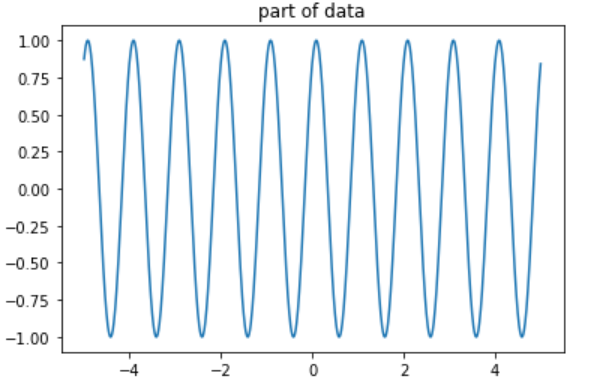
\includegraphics[width=6cm, height=4cm]{2022-05-06 21-47-03屏幕截图}

现在我们有了数据,我们实际上想要实现什么?好吧,只是我们希望 LSTM 从我们将提供给它的一组数据窗口大小的数据中学习正弦波,并希望我们可以让 LSTM 预测该系列中接下来的 N 步,它会继续输出正弦波。

我们将首先将数据从 CSV 文件转换并加载到 pandas 数据帧,然后将其用于输出将馈送 LSTM 的 numpy 数组。Keras LSTM 层的工作方式是采用 3 维(N、W、F)的 numpy 数组,其中 N 是训练序列的数量,W 是序列长度,F 是每个序列的特征数。我们选择使用 50 的序列长度(读取窗口大小),这样网络就可以瞥见每个序列的正弦波形状,因此希望能够自学根据之前收到的窗口。

为了加载这些数据,我们在代码中创建了一个 DataLoader 类来为数据加载层提供抽象。您会注意到,在初始化 DataLoader 对象时,会传入文件名,以及一个拆分变量,该变量确定用于训练与测试的数据百分比,以及一个允许选择一列或多列数据的列变量用于单维或多维分析。

{\heiti \subsection{二级标题 *字体为5号黑体*标题2} }
\subsubsection{三级标题 *字体为5号宋体*标题3}
*
\begin{figure}[htbp]
\centerline{
\includegraphics[width=3.15in,height=1.98in]{CJC1.pdf}}
图X\quad  图片说明 *字体为小5号,图片应为黑白图,图中的子图要有子图说明*
\label{fig1}
\end{figure}

\begin{table}[htbp]
\centering {\heiti 表X\quad 表说明 *表说明采用黑体* }
\vspace {-2.5mm}
\begin{center}
\begin{tabular}{ll}
\toprule
*示例表格*&*第1行为表头,表头要有内容* \\
\hline
&
 \\
&
 \\
&
 \\
&
 \\
\bottomrule
\end{tabular}
\label{tab1}
\end{center}
\end{table}

\heiti 过程X. \quad 过程名称

{\zihao{5-}*《计算机学报》的方法过程描述字体为小5号宋体,IF、THEN等伪代码关键词全部用大写字母,变量和函数名称用斜体*}


\heiti 算法\textbf{Y} .\quad 算法名称.
\zihao{5-}{

\noindent 输入:{\ldots} {\ldots}

\noindent 输出:{\ldots} {\ldots}

*《计算机学报》的算法描述字体为小5号宋体, IF、THEN等伪代码关键词全部用大写字母,变量和函数名称用斜体*}

\vspace {3mm}
\zihao{5}{
\noindent \heiti 致\quad 谢 \quad  \kaishu   *致谢内容.* 致谢 }


\vspace {5mm}
\centerline
{\zihao{5}
\heiti 参~考~文~献 }

% \begin{thebibliography}{99}
% \zihao{5-} \addtolength{\itemsep}{-1em}
% \vspace{1.5mm}

% \bibitem[1]{1}
% 网上的文献(举例:The Cooperative
% Association for Internet Data Analysis(CAIDA),http://www.caida.org/data
% 2010,7,18) \textbf{*请采用脚注放于正文出现处,每页的脚注从1开始编序号*}\footnote{The Cooperative Association for Internet Data
% Analysis (CAIDA), http://www.caida.org/data 2010, 7, 18}

% \bibitem[2]{2} 中文的参考文献需给出中英文对照。形式如[3]。

% \bibitem[3]{3} Zhou Yong-Bin, Feng Deng-Guo. Design and analysis of cryptographic
% protocols for RFID. Chinese Journal of Computers, 2006, 29(4): 581-589 (in
% Chinese) \newline
% (周永彬, 冯登国. RFID安全协议的设计与分析. 计算机学报, 2006, 29(4): 581-589)

% \bibitem[4]{4} 期刊、会议、书籍名称不能用缩写。

% \bibitem[5]{5} 作者(外国人姓在前,名在后可缩写, 后同).
% 题目(英文题目第一字母大写,其它均小写):副标题(如果有). 刊名(全称), 年,
% 卷(期): 页码 \textbf{*期刊论文格式*}

% \bibitem[6]{6}作者.
% 文章题目(英文题目第1字母大写,其它均小写):副标题(如果有)//Proceedings of
% the {\ldots} (会议名称). 会议召开城市, 会议召开城市所在国家, 年: 页码
% \textbf{*会议论文集论文格式*}

% \bibitem[7]{7}作者. 文章题目(英文题目第一字母大写, 其它均小写):
% 副标题(如果有)//编者. 文集标题. 出版地: 出版社, 出版年: 页码
% \textbf{*文集格式*}

% \bibitem[8]{8}作者. 书名: 副标题(如果有). 版次(初版不写). 出版社地点: 出版社,
% 出版年 \textbf{*书籍格式*}

% \bibitem[9]{9}作者. 文章题目[博士学位论文/硕士学位论文]. 单位名称,单位地点, 年
% \textbf{*学位论文格式*}

% \bibitem[10]{10}作者. 文章题目(英文题目第一字母大写,其它均小写). 单位地点: 单位,
% 技术报告: 报告编号, 年 \textbf{*技术报告*}

% \bibitem[11]{11}专利拥有人. 专利名称,专利授权国家,专利授权日期
% \textbf{*技术专利*}
%   \end{thebibliography}

\begin{strip}
\end{strip}

\noindent {\zihao{5}\bf{附录X}.}

{\zihao{5-}\setlength\parindent{2em}
*\textbf{附录内容}置于此处,字体为小5号宋体。附录内容包括:\textbf{详细的定理证明、公式推导、原始数据}等*}

\begin{strip}
\end{strip}

\begin{biography}[yourphotofilename.jpg]
\noindent
\textbf{First A. Author}\ \ *计算机学报第1作者提供照片电子图片,尺寸为1寸。英文作者介绍内容包括:出生年,学位(或目前学历),职称,主要研究领域(\textbf{与中文作者介绍中的研究方向一致}).*
*字体为小5号Times New Roman*

\end{biography}

\begin{biography}[yourphotofilename.jpg]
\noindent
\textbf{Second B. Author} *英文作者介绍内容包括:出生年,学位(或目前学历),职称,主要研究领域(\textbf{与中文作者介绍中的研究方向一致})。*
*字体为小5号Times New Roman*
\end{biography}
\begin{strip}
\end{strip}
\zihao{5}
\noindent \textbf{Background}

\zihao{5-}{
\setlength\parindent{2em}
*论文背景介绍为\textbf{英文},字体为小5号Times New Roman体*

论文后面为400单词左右的英文背景介绍。介绍的内容包括:

本文研究的问题属于哪一个领域的什么问题。该类问题目前国际上解决到什么程度。

本文将问题解决到什么程度。

课题所属的项目。

项目的意义。

本研究群体以往在这个方向上的研究成果。

本文的成果是解决大课题中的哪一部分,如果涉及863$\backslash $973以及其项目、基金、研究计划,注意这些项目的英文名称应书写正确。}

 
\end{document}


